	
\documentclass[varwidth, border=15pt]{standalone}
\usepackage{caption}
\usepackage{subcaption}
\usepackage[labelformat=parens,labelsep=quad,skip=3pt]{caption}
\usepackage{graphicx}

\usepackage{tabularx} % Addition
\usepackage{multirow} % Addition
\usepackage{booktabs} % Addition
\usepackage[export]{adjustbox}

\begin{document}
\begin{figure}[t]
	\centering

\begin{tabularx}{0.5\textwidth}{llrrr}
& &  \rotatebox{90}{Bert$_{reference}$} &  \rotatebox{90}{Bert-ptrn$_{reference}$} &  \rotatebox{90}{Bert-ptrn$_{pero-ocr}$} \\
\midrule
\multirow{3}{*}{\rotatebox{90}{Test set}} & reference & 96.4  & \textbf{96.5} &                    95.2 \\
& pero-ocr  & 92.5 &                     92.9 &                   \textbf{94.1} \\
& tesseract &  90.5 &                     90.8 &                    \textbf{91.2} \\
\bottomrule
\end{tabularx}
     \begin{subfigure}{1\textwidth}
     \centering
         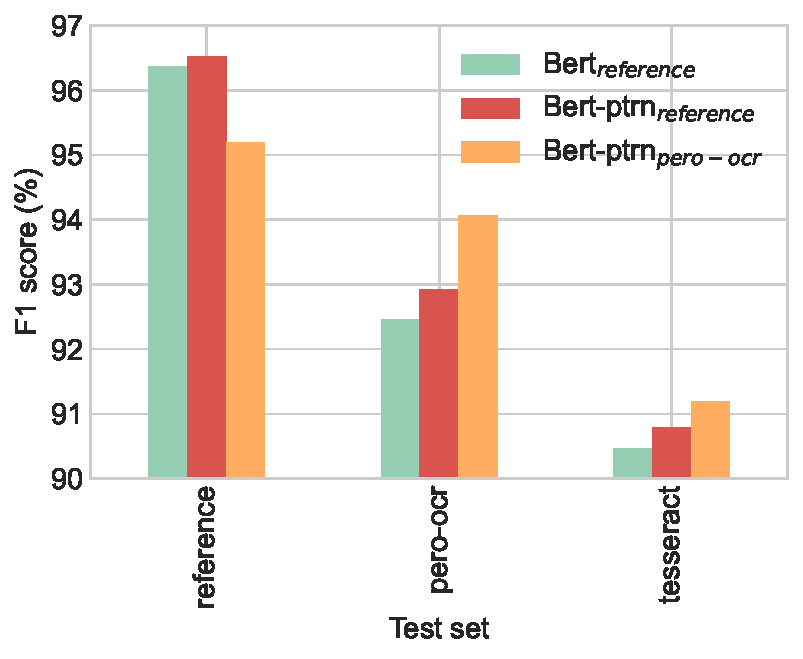
\includegraphics[width=0.8\textwidth,valign=t]{experiment_2_f1_with_noise_graph.pdf}
     \end{subfigure}
\end{figure}
\end{document}

%      \caption{F1 scores (in \%) of NER predictions in presence of OCR noise in the training and testing data, either manually corrected or OCRed with Pero-OCR and Tesseract. The type of examples used to train the NER task is noted in indice after the model name (e.g. Bert$_{reference}$). Results show that the best performances on OCRed entries are obtained when the BERT model has been pretrained and fine-tuned for NER on examples affected with similar OCR errors.}